\IfFileExists{llncs.cls}{%
  \documentclass[runningheads]{llncs}
}{%
  \documentclass[10pt]{article}
}

\makeatletter
\@ifclassloaded{llncs}{}{\usepackage[a4paper,margin=2.8cm]{geometry}}
\makeatother
\usepackage{graphicx}
\usepackage{booktabs}
\usepackage{array}
\usepackage{multirow}
\usepackage{makecell}
\usepackage{siunitx}
\usepackage{amsmath}
\usepackage{amssymb}
\usepackage{url}
\usepackage{placeins}
\makeatletter
\let\catad@thebibliography\thebibliography
\renewcommand{\thebibliography}[1]{%
  \catad@thebibliography{#1}%
  \fontsize{8.6pt}{10pt}\selectfont
}
\makeatother
\setlength{\emergencystretch}{2em}

\providecommand{\institute}[1]{\date{#1}}
\providecommand{\titlerunning}[1]{}
\providecommand{\authorrunning}[1]{}
\graphicspath{{../figures/}{figures/}}

\newcommand{\maybeinput}[1]{%
  \IfFileExists{#1}{\input{#1}}{}%
}

\title{CAT-AD: Constrained Adversarial Training for Robust ADS-B Trajectory Anomaly Detection}
\titlerunning{CAT-AD: Robust ADS-B Trajectory Anomaly Detection}
\author{Anonymous Authors}
\authorrunning{Anonymous Authors}
\institute{Anonymous Institution}

\begin{document}
\maketitle

\begin{abstract}
Automatic Dependent Surveillance--Broadcast (ADS-B) trajectory detectors can be evaded by perturbing anomalous trajectories toward the normal class, while norm-bounded evaluation can overlook aircraft-motion feasibility.
Under a targeted anomalous-to-normal evasion threat model, we propose constrained adversarial training for anomaly detection (CAT-AD), combining physically constrained adversarial training with prediction- and feature-level consistency.
We evaluate five matched aircraft-level splits/seeds using norm-bounded projected gradient descent without physical constraints (Norm-bounded PGD) and two physically constrained PGD (Phys-PGD) variants.
We report physically valid attack success conditioned on pre-attack-valid samples (PV-ASR$\mid V_0$) to separate successful evasion from inherited invalidity.
Relative to BiLSTM-ERM, CAT-AD reduces PV-ASR$\mid V_0$ from $0.9336$ to $0.0002$ under projection-based Phys-PGD and from $0.9306$ to $0.0002$ under penalty-based Phys-PGD.
Under the same unperturbed-detection protocol, CAT-AD achieves an F1-score of $0.908$ and a false alarm rate (FAR) of $0.026$; three protocol-aligned ADS-B detectors from 2021--2022 achieve F1-scores of $0.447$--$0.577$ and FARs of $0.422$--$0.515$.
All robustness claims are limited to the evaluated perturbation settings and threat model.
\end{abstract}

\keywords{ADS-B \and trajectory anomaly detection \and adversarial training \and physical constraints \and robust machine learning}

\section{Introduction}
\label{sec:introduction}

Automatic Dependent Surveillance--Broadcast (ADS-B) trajectory streams are increasingly used for situational awareness, airspace monitoring, and downstream safety analytics.
At the same time, ADS-B messages are unauthenticated at the broadcast layer, which makes trajectory-level anomaly detection an important defensive component~\cite{strohmeier2015security}.
Recent neural detectors can fit normal and abnormal trajectory patterns, but strong clean-set accuracy is not sufficient when an attacker can perturb anomalous trajectories to look normal to the detector.
This paper therefore studies targeted anomalous-to-normal evasion against ADS-B trajectory anomaly detection.

We focus on a practical robustness question: can adversarial training improve detector robustness without relying on perturbations that are physically implausible for aircraft motion?
To answer this question, we evaluate norm-bounded projected gradient descent (PGD) without physical constraints and physically constrained PGD variants.
We report the F1-score and false alarm rate (FAR) together with attack success rate (ASR), paired pre/post physical violation rates (PVR), and physically valid ASR conditioned on trajectories that are valid before attack (PV-ASR$\mid V_0$).
This conditioning separates violations inherited from the source trajectory from violations introduced by the attack.

The contributions are:
\begin{itemize}
\item A constrained adversarial training framework for ADS-B trajectory anomaly detection that combines physically constrained adversarial examples with prediction- and representation-level consistency.
\item A targeted anomalous-to-normal evaluation protocol with paired pre/post feasibility flags that separates inherited invalidity, attack-introduced violations, and physically valid evasion.
\item A reproducible multi-seed benchmark pipeline with aircraft-level splits, a same-protocol comparison against three recent (2021--2022) ADS-B detectors, artifact hashes, paired comparisons, and strict publication gates.
\end{itemize}

\section{Related Work}
\label{sec:related_work}

\paragraph{ADS-B Security and Trajectory Data.}
ADS-B has been widely studied as a security-sensitive broadcast protocol because receivers cannot directly authenticate message origin or integrity~\cite{strohmeier2015security}.
OpenSky demonstrated that large-scale crowdsourced ADS-B collection can support reproducible air-traffic research~\cite{schaefer2014opensky}.
Sensor-network defenses such as wireless witnessing use geographically distributed receivers to cross-validate ADS-B reports and detect Global Positioning System (GPS) spoofing, ADS-B spoofing, and Sybil attacks~\cite{jansen2021trust}.
These properties motivate data-driven detectors, but they also require careful split design: aircraft-level leakage can make clean accuracy look stronger than deployment robustness.

\paragraph{ADS-B Anomaly Detection.}
Prior work has studied autoencoder, recurrent, and hybrid models for detecting abnormal ADS-B trajectories or message streams.
Fried and Last use recurrent autoencoders over trajectory variables and their temporal differences~\cite{fried2021autoencoders}; Luo et al. combine recurrent variational reconstruction residuals with a support-vector data-description boundary~\cite{luo2021vaesvdd}; and Chevrot et al. introduce a contextual autoencoder with a shared recurrent encoder and flight-phase-specific decoders~\cite{chevrot2022cae}.
Section~\ref{subsec:published_comparison_protocol} operationalizes these designs, published in 2021--2022 within its July 2019--July 2026 window, under one split, window, threshold-selection, and test protocol rather than copying numbers from incompatible datasets.
Recent ADS-B intrusion-detection work also explores realistic low-altitude attack scenarios, attack detection and recovery, attack-vector benchmarks, deep attack-type classifiers, lightweight intrusion detection system (IDS) designs, adversarial-perturbation detectors, physics-consistent trajectory anomaly detection, transformer and extended long short-term memory (xLSTM) transfer-learning models, ADS-B data-security analyses, and broader ADS-B or ADS-B/Remote Identification (Remote ID) security taxonomies~\cite{pirolley2026lowaltitude,yue2026ocren,cevik2025adsbanomalydetection,ahmed2025adsbanomalous,ahmed2026lightweightadsb,zhong2026rdpaadsb,zhao2026imdmpc,ngamboe2025adsbids,khan2025surveyadsbsecurity,zhang2025adsbdatasecurity,shi2026securityadsbrid,ahmed2026secureairtraffic}.
Surveys further link trajectory outliers to operational speed, altitude, and heading behavior~\cite{wu2026reviewtrajectory}.
These defenses often emphasize clean or injected anomalies; CAT-AD instead tests adaptive targeted optimization toward the normal decision region.

\paragraph{Adversarial Robustness.}
Adversarial examples and adversarial training are well established in deep learning~\cite{goodfellow2015explaining,madry2018towards}.
Security-oriented evaluations emphasize that robustness claims require strong attacks and careful threat-model definition~\cite{carlini2017towards,athalye2018obfuscated}.
Following this principle, our evaluation reports Norm-bounded PGD together with physically constrained attacks and explicitly limits claims to the evaluated perturbation budget, physical constraints, and target class.
ADS-B-specific adversarial work has already shown that deep ADS-B anomaly detectors can be attacked, including the Time Neighborhood Accumulation Iteration Fast Gradient Sign Method (TNAI-FGSM) and adversarial-training baselines~\cite{luo2024adversarialadsb}.
Therefore, this paper does not claim that ADS-B anomaly detection, recurrent detectors, PGD attacks, adversarial examples, or adversarial training are new.
To the best of our knowledge, the novelty claim is narrower: CAT-AD studies targeted anomalous-to-normal evasion for ADS-B trajectory anomaly detection through physically constrained adversarial training, reports paired pre/post validity and exact PV-ASR conditioned on valid starts rather than ASR alone, and verifies the resulting claims with a multi-seed publication gate.

\paragraph{Positioning against Prior Work.}
Table~\ref{tab:positioning} summarizes the boundary of the contribution.
The table is intended to make the novelty claim falsifiable: a prior method would subsume CAT-AD only if it jointly covered the ADS-B trajectory setting, targeted anomalous-to-normal evasion, physically constrained attack generation or training, valid-start-conditioned physical evasion metrics, consistency regularization, and multi-seed reproducibility checks.

\begin{table*}[t]
\centering
\footnotesize
\setlength{\tabcolsep}{2pt}
\renewcommand{\arraystretch}{1.08}
\caption{Coverage relative to representative prior work. A check mark denotes direct coverage, ``partial'' incomplete coverage, and a dash no identified coverage; definitions and citations for each line of work are given in Sect.~\ref{sec:related_work}.}
\label{tab:positioning}
\begin{tabular}{@{}p{0.232\textwidth}>{\centering\arraybackslash}p{0.097\textwidth}>{\centering\arraybackslash}p{0.097\textwidth}>{\centering\arraybackslash}p{0.097\textwidth}>{\centering\arraybackslash}p{0.105\textwidth}>{\centering\arraybackslash}p{0.097\textwidth}>{\centering\arraybackslash}p{0.097\textwidth}@{}}
\toprule
Line of work &
\makecell{ADS-B\\traj.} &
\makecell{Target\\evasion} &
\makecell{Phys.\\bounds} &
\makecell{PV-ASR} &
\makecell{Consist.\\reg.} &
\makecell{Reprod.\\gate} \\
\midrule
ADS-B security and data infrastructure & partial & partial & partial & -- & -- & -- \\
ADS-B trajectory anomaly detectors & $\checkmark$ & -- & partial & -- & -- & -- \\
Recent ADS-B detection, recovery, and IDS & partial & partial & partial & -- & -- & -- \\
ADS-B adversarial attacks & $\checkmark$ & $\checkmark$ & -- & -- & partial & -- \\
General adversarial robustness & -- & $\checkmark$ & -- & -- & partial & partial \\
CAT-AD & $\checkmark$ & $\checkmark$ & $\checkmark$ & $\checkmark$ & $\checkmark$ & $\checkmark$ \\
\bottomrule
\end{tabular}
\par\smallskip
\begin{minipage}{0.98\textwidth}
\footnotesize Abbreviations: traj., trajectory; Consist. reg., consistency regularization; Reprod. gate, reproducibility gate.
\end{minipage}
\end{table*}

\section{Method}
\label{sec:method}

\subsection{Trajectory Detector}
\label{subsec:detector}

Each trajectory window is represented by six raw physical variables and six temporal-difference variables, yielding a 12-dimensional feature vector per time step.
The detector is a two-layer bidirectional long short-term memory (BiLSTM) network followed by a multilayer classification head.
The model outputs logits for the normal class and anomalous class.
Let $f_\theta(x)$ denote the detector and let $p_\theta(y=1\mid x)$ be the predicted anomalous probability.
The decision threshold is selected on the validation split and then held fixed for test evaluation.

\subsection{Threat Model and Physically Constrained Attacks}
\label{subsec:threat_model}

The attack perturbs anomalous windows only and targets the normal class.
Given an anomalous trajectory $x$ with label $y=1$, the targeted attack searches for $x'$ that is classified as normal while remaining within an $\ell_\infty$ budget in normalized feature space.
Norm-bounded PGD is the digital reference attack: it enforces the normalized $\ell_\infty$ perturbation budget but no aircraft-motion constraints.
Projection-based physically constrained PGD (Projection-based Phys-PGD) hard-projects every intermediate update into both the normalized $\ell_\infty$ budget and the evaluated per-field displacement bounds for position (latitude and longitude), altitude, ground speed, and heading.
Penalty-based physically constrained PGD (Penalty-based Phys-PGD) optimizes a targeted cross-entropy (CE) classification loss augmented with differentiable penalties for kinematic violations:
\begin{equation}
  \min_{x'} \mathcal{L}_{\mathrm{CE}}(f_\theta(x'), y_t=0)
  + \lambda_{\mathrm{phys}}\mathcal{R}_{\mathrm{phys}}(x'),
  \quad \|x'-x\|_\infty \le \epsilon .
\end{equation}
The physical penalty covers position, altitude, speed, and heading-change constraints.
All physical feasibility metrics retain paired flags for each attacked anomalous sample before and after perturbation.

\subsection{CAT-AD Training Objective}
\label{subsec:catad}

CAT-AD trains on unperturbed trajectories and physically constrained adversarial trajectories; $x_{\mathrm{adv}}$ denotes the adversarial counterpart of an unperturbed trajectory $x$.
For anomalous samples, the adversarial training term uses the original anomalous label during detector training, while the attack generator targets the normal class.
The training objective is
\begin{equation}
  \mathcal{L}_{\mathrm{CAT}} =
  \mathcal{L}_{\mathrm{CE}}(f_\theta(x), y) + \mathcal{R}_{\mathrm{rob}}(x,x_{\mathrm{adv}}),
\end{equation}
where the robustness regularizer uses Kullback--Leibler (KL) divergence and mean squared error (MSE), and is defined using the softmax temperature $T>0$,
$p^{(T)}(z)=\operatorname{softmax}(f_\theta(z)/T)$,
$\bar h(z)=h_\theta(z)/\|h_\theta(z)\|_2$, and a stop-gradient operator
$\operatorname{sg}[\cdot]$. For compactness, let $q=p^{(T)}(x)$,
$q_{\mathrm{adv}}=p^{(T)}(x_{\mathrm{adv}})$,
$r=\bar h(x)$, and $r_{\mathrm{adv}}=\bar h(x_{\mathrm{adv}})$. Then
\begin{equation}
  \mathcal{R}_{\mathrm{rob}} =
  \lambda_{\mathrm{adv}}\mathcal{L}_{\mathrm{CE}}(f_\theta(x_{\mathrm{adv}}), y)
  + \lambda_{\mathrm{out}}T^2\mathrm{KL}\!\left(\operatorname{sg}[q]\,\|\,q_{\mathrm{adv}}\right)
  + \lambda_{\mathrm{rep}}\operatorname{MSE}\!\left(r_{\mathrm{adv}},\operatorname{sg}[r]\right) .
\end{equation}
Here $h_\theta(\cdot)$ is the LSTM representation before the classifier head; the implementation uses $T=2$.
The adversarial and consistency terms are evaluated only on anomalous samples.

\paragraph{Method--Implementation Traceability.}
The archived implementation maps the objective above to unperturbed CE, anomalous-only adversarial CE, output-level KL consistency, and BiLSTM-representation MSE consistency.
The generator targets the normal class, whereas training retains the original anomalous labels; the method--implementation audit checks this boundary against the code, benchmark manifest, and seed logs.

\section{Experimental Setting}
\label{sec:experimental_setting}

The main experiments compare a BiLSTM detector trained by empirical risk minimization (BiLSTM-ERM) with CAT-AD on the same aircraft-level train, validation, and test split.
Fairness controls are applied throughout this comparison: both detectors use the same BiLSTM architecture, the same train, validation, and test loaders, the same validation-only threshold-selection protocol, and the same test-time attack/evaluation settings.
The paired seed-wise comparisons match each CAT-AD result to a BiLSTM-ERM run using the same split seed.
The unperturbed setting uses the same mixed test set containing both normal and anomalous trajectories, but no adversarial perturbation is applied.
For adversarial settings, the attack is a targeted anomalous-to-normal evasion attack: adversarial samples are generated from anomalous trajectories with target label $y_t=0$, while the detector is evaluated against the original label $y$.
ASR is therefore reported only for adversarial settings and denotes the fraction of attacked anomalous samples classified as normal.

\subsection{Published-Model Comparison Protocol}
\label{subsec:published_comparison_protocol}

We use a rolling seven-year publication window (July 2019--July 2026).
Eligible comparators are peer-reviewed decoded-trajectory ADS-B anomaly detectors with sufficiently specified architectures and training objectives and no extra-sensor requirement.
We select three representative, non-exhaustive, protocol-aligned baselines: the 2021 Fried--Last Differenced LSTM Autoencoder (Fried--Last Differenced LSTM-AE)~\cite{fried2021autoencoders}; the 2021 recurrent variational autoencoder (VAE) with a radial basis function (RBF) support vector data description (SVDD) boundary, denoted VAE--SVDD~\cite{luo2021vaesvdd}; and the 2022 Contextual Autoencoder (Contextual AE) with climb, cruise, and descent decoders~\cite{chevrot2022cae}.
The comparison uses the same five aircraft-level splits, normalized 15-step windows, validation-only maximum-F1-score threshold selection, and injected test windows as BiLSTM-ERM and CAT-AD.
The defining architecture and one-class decision rule of each published method are retained, but their original datasets, feature sets, sequence lengths, and frameworks are replaced by this common protocol; the resulting values are therefore controlled reimplementations, not exact reproductions of the source papers' reported numbers.
Consistent with their objectives, the three one-class methods train on the normal-only view of the shared training windows, whereas the supervised methods use the corresponding labeled view.

The cross-family table reports unperturbed detection metrics only.
Applying the fixed five-step classifier-PGD evaluator to reconstruction models failed a step-size sanity check: a smaller step reversed the apparent zero-ASR result, demonstrating overshoot rather than robustness.
We therefore exclude those attack outputs instead of interpreting a failed optimizer as evidence for the one-class methods; adversarial claims remain restricted to the pre-specified BiLSTM-ERM--CAT-AD comparison.

The benchmark dataset is an offline decoded ADS-B sample covering one Coordinated Universal Time (UTC) day.
The raw comma-separated values (CSV) file contains 217,148 rows and 20 raw aircraft identifiers; after model-field selection and physical sanity filtering, the publication preflight report records 75,238 rows and 19 filtered aircraft.
All results are therefore scoped to this archived sample, the aircraft-level splits generated from it, and the evaluated perturbation budgets.

The perturbation settings include Norm-bounded PGD, Projection-based Phys-PGD, and Penalty-based Phys-PGD.
Norm-bounded PGD is the digital perturbation reference setting.
Projection-based Phys-PGD imposes physical projection after gradient updates, whereas Penalty-based Phys-PGD integrates physical-constraint penalties into the attack objective.
The physical feasibility analysis is computed at the sample level: a trajectory is counted as violating if it violates any one of the position, altitude, ground-speed, or heading constraints.
Let $\mathcal{A}$ denote attacked anomalous samples, $s_i=\mathbf{1}[\hat{y}(x'_i)=0]$ denote targeted evasion success, and $v_i^0$ and $v_i^1$ denote physical-violation flags before and after attack.
Define the valid-start set $V_0=\{i\in\mathcal{A}:v_i^0=0\}$.
We report
\begin{equation}
\mathrm{Pre\text{-}PVR}=|\mathcal{A}|^{-1}\sum_i v_i^0,
\quad
\mathrm{Post\text{-}PVR}=|\mathcal{A}|^{-1}\sum_i v_i^1,
\end{equation}
and the paired conditional metrics
\begin{equation}
\mathrm{New\text{-}PVR}\mid V_0 = |V_0|^{-1}\sum_{i\in V_0}v_i^1,
\qquad
\mathrm{ASR}\mid V_0 = |V_0|^{-1}\sum_{i\in V_0}s_i,
\end{equation}
and
\begin{equation}
\mathrm{PV\text{-}ASR}\mid V_0 = |V_0|^{-1}\sum_{i\in V_0}s_i(1-v_i^1).
\end{equation}
Thus PV-ASR$\mid V_0$ is an exact per-sample intersection and is not estimated as $(\mathrm{ASR}\mid V_0)(1-\mathrm{New\text{-}PVR}\mid V_0)$, because attack success and physical validity need not be independent.

\subsection{Statistical Protocol}
\label{subsec:statistical_protocol}

For publication-grade claims, the experiment runner repeats the full training, validation, and test procedure over independent seeds and aggregates results across seeds.
The benchmark records the conda environment, package snapshot, dataset hash, code fingerprint, hyperparameter snapshot, aircraft-level split audits, per-seed logs, and 256-bit Secure Hash Algorithm (SHA-256) checksums for generated artifacts.
The strict publication gate requires at least five independent seeds, full-data usage, deterministic execution metadata, physical metrics for attack settings, and positive primary CAT-AD robustness claims.
The archived benchmark ran on an NVIDIA GeForce RTX 4070 Laptop graphics processing unit (GPU) with CUDA 12.4 and PyTorch 2.5.1; resumable per-seed records preserve the runtime boundary and source signature.
The compute-resource audit verifies the \texttt{testtorch} conda environment and the per-seed logs.
Paired comparisons use seed-wise differences between CAT-AD and BiLSTM-ERM; positive improvement means CAT-AD is better.
For the six primary claims, the paired improvement direction is positive in all five seeds; this consistency check is reported as robustness evidence, not as a substitute for broader datasets or additional attack families.

\paragraph{Statistical Interpretation.}
With five seeds, exact sign-flip p-values are coarse, so the paired table is interpreted primarily through effect sizes, confidence intervals, win rates, and consistency of paired improvements.
The adjusted p-values and Benjamini--Hochberg (BH) false-discovery-rate q-values are reported for transparency but are not interpreted as conclusive hypothesis-test evidence.
The reported Student-$t$ intervals are unbounded and can therefore extend outside $[0,1]$ for bounded metrics; they are not clipped after estimation.
The claims therefore remain directional and artifact-checked within the evaluated seeds, perturbation budgets, and threat model.

\subsection{Attack Evaluation Sanity Checks}
\label{subsec:attack_sanity}

We include attack sanity checks to reduce the risk that robustness results are an artifact of weak attacks or gradient masking.
The PGD implementation freezes dropout during attack-gradient computation, applies targeted anomalous-to-normal attacks only to anomalous windows, and keeps the original evaluation labels fixed.
Unit tests check targeted PGD direction, anomalous-only attack application, hard physical projection, penalty-based Phys-PGD diagnostics and budget bounds, paired pre/post feasibility, and exact conditional PV-ASR.
The attack configuration is fixed before paired comparison: PGD uses five steps with step size $0.03$ under evaluation budget $0.1$, the benchmark manifest records these hyperparameters, and the epsilon-sensitivity sweep evaluates the two physical attack families across additional budgets.
The evaluated attacks also produce high ASR against BiLSTM-ERM under Norm-bounded PGD, Projection-based Phys-PGD, and Penalty-based Phys-PGD, which indicates that the attacks are nontrivial for the baseline detector.
This sanity statement concerns the two supervised detectors sharing the classifier objective; it is not used to claim attack adequacy for the heterogeneous one-class scores in Table~\ref{tab:literature_detection}.
These checks do not establish a formal robustness certificate or coverage of all adaptive attackers; they support the narrower claim that CAT-AD is robust under the evaluated attack families and perturbation budgets.

\input{../outputs/tables/table_experimental_setup.tex}

\input{../outputs/publication_benchmark/data_split_audit.tex}

\section{Main Robustness Results}
\label{sec:main_results}

Unperturbed detection performance alone does not characterize targeted evasion robustness.
BiLSTM-ERM achieves strong unperturbed detection performance, but its F1-score collapses under Norm-bounded PGD and remains vulnerable under physically constrained attacks.
CAT-AD maintains high F1-score and low ASR across the evaluated adversarial settings, indicating robustness against targeted anomalous-to-normal evasion within the evaluated threat model.
The paired improvement direction is positive in all five seeds for the six primary claims, but the exact two-sided sign-flip p-value is 0.0625 and no primary row is significant after Holm correction; we therefore treat the results as large, consistent effect estimates rather than conclusive population-level hypothesis tests.
Table~\ref{tab:multiseed_summary} reports the exact multi-seed means and uncertainty, while Fig.~\ref{fig:robustness_comparison} provides the corresponding visual comparison with 95\% confidence intervals.

\IfFileExists{../outputs/tables/table_multiseed_summary.tex}{%
Table~\ref{tab:paired_multiseed_comparison} reports paired seed-wise improvements, adjusted p-values, BH q-values, and effect sizes.
\maybeinput{../outputs/tables/table_multiseed_summary.tex}
\maybeinput{../outputs/tables/table_paired_multiseed_comparison.tex}
}{}

\subsection{Same-Protocol Comparison with Recent Published ADS-B Detectors}
\label{subsec:published_detection_results}

Table~\ref{tab:literature_detection} reports the recent published-model comparison under the stated window and common unperturbed-detection protocol.
CAT-AD obtains an F1-score of $0.908\pm0.023$ and a FAR of $0.026\pm0.006$.
Fried--Last Differenced LSTM-AE, VAE--SVDD, and Contextual AE obtain F1-scores of $0.577$, $0.447$, and $0.569$, respectively, with substantially higher FARs of $0.422$, $0.515$, and $0.453$.
Relative to CAT-AD, their mean paired F1-score gaps are $0.332$, $0.461$, and $0.339$; CAT-AD has higher F1-scores and lower FARs on all five matched aircraft splits for every comparator, including BiLSTM-ERM.
The one-class models retain moderate-to-high recall but reject many normal windows, showing that their lower F1 is primarily associated with poor precision/FAR trade-offs under the shared validation threshold.
VAE--SVDD is also split-sensitive (FAR interval half-width $0.550$), so its mean should not be read as a stable cross-dataset ranking.

\input{../outputs/literature_benchmark/table_literature_detection.tex}

\begin{figure*}[t]
\centering
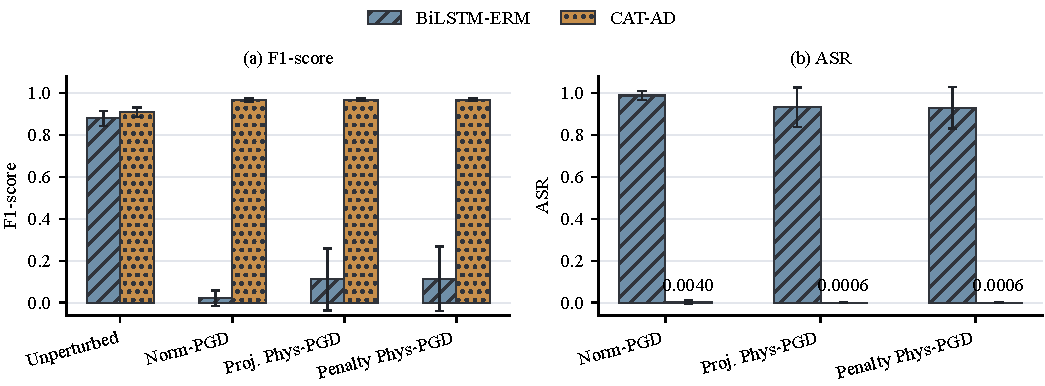
\includegraphics[width=\textwidth]{fig_main_robustness.pdf}
\caption{Five-run robustness comparison between BiLSTM-ERM and CAT-AD. Bars show means and whiskers show unbounded 95\% Student-$t$ confidence intervals over matched aircraft splits/seeds; hatching preserves model identity in grayscale. Exact values are reported in Table~\ref{tab:multiseed_summary}.}
\label{fig:robustness_comparison}
\end{figure*}

\section{Physical Feasibility Analysis}
\label{sec:physical_feasibility}

High attack success is not sufficient to establish a realistic trajectory-level threat.
The feasibility results in Table~\ref{tab:physical_feasibility} show that ASR alone can overestimate the practical threat of norm-bounded digital perturbations without physical constraints.
Physically constrained attacks provide a stricter view of evasion by measuring whether successful perturbations remain compatible with ADS-B trajectory constraints for samples that were valid before attack.
Across five seeds, the valid-start rate is 0.8423 on average. Projection-based Phys-PGD has zero New-PVR$\mid V_0$ for both models while attaining baseline PV-ASR$\mid V_0=0.9336$; CAT-AD reduces it to 0.0002. Penalty-based Phys-PGD yields corresponding values of 0.9306 and 0.0002, with mean New-PVR$\mid V_0$ at most 0.0001.
Figure~\ref{fig:physical_valid_asr}(a) summarizes conditional PV-ASR, highlighting that CAT-AD substantially suppresses physically valid anomalous-to-normal evasion without relying on newly invalid trajectories.
Pre- and post-attack PVR should therefore be read as physical-validity diagnostics; the primary robustness claims are tied to F1, ASR, and PV-ASR$\mid V_0$ under the evaluated attacks.

\input{../outputs/tables/table_physical_feasibility.tex}

\section{Ablation Summary and Sensitivity Analysis}
\label{sec:ablation_summary}

The ablation results should be read as a trade-off analysis rather than as a ranking in which one configuration is best on every metric.
Table~\ref{tab:ablation} includes strong adversarial-training baselines beyond ERM: norm-bounded PGD adversarial training (PGD-AT), projection-based Phys-PGD adversarial training (Projection Phys-PGD-AT), and penalty-based Phys-PGD adversarial training (Penalty Phys-PGD-AT).
These baselines are intentionally retained in the paper because they make the comparison harder: physical adversarial training alone can already be strong in the single-seed auxiliary table.
Prediction consistency and feature consistency are introduced to improve output-level and representation-level stability; they are not intended to guarantee the best value on every individual metric.
The variant without differential trajectory features has low ASR and PV-ASR, but its FAR increases sharply, indicating that low attack success is not a valid robustness gain when normal trajectories are rejected at an unacceptable rate.
We keep this negative ablation visible because it constrains the interpretation of the method: differential motion features are required for a useful detector in this experimental setting.
Table~\ref{tab:ablation} therefore supports CAT-AD as a balanced design under the evaluated perturbation settings; it does not claim that CAT-AD dominates every metric in the auxiliary ablation table.

\input{../outputs/tables/table5_ablation_study.tex}

Perturbation-budget sensitivity further supports this interpretation.
As the perturbation budget increases, BiLSTM-ERM suffers a clear F1-score drop under both physically constrained attacks, whereas CAT-AD remains stable across the evaluated budgets.
This sensitivity result, shown in Fig.~\ref{fig:epsilon_sensitivity}(b,c), should be interpreted only for the evaluated budget range and attack settings.

\begin{figure*}[t]
\centering
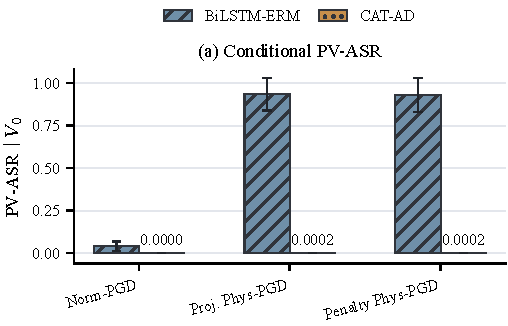
\includegraphics[width=0.62\textwidth]{fig_physical_valid_asr.pdf}
\par\smallskip
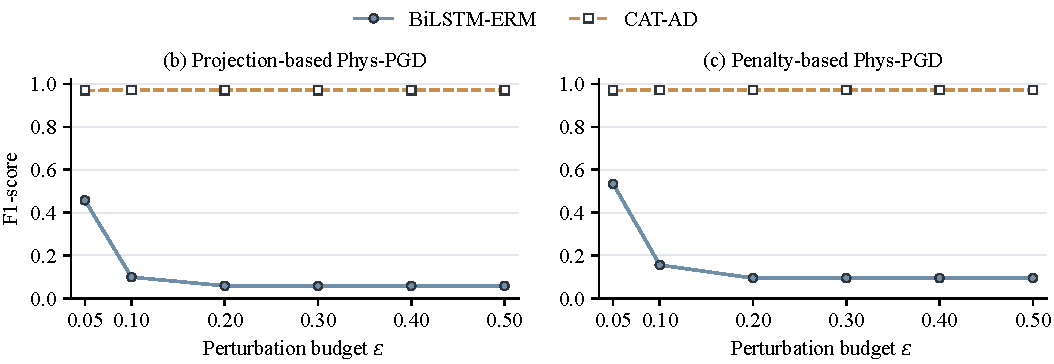
\includegraphics[width=0.90\textwidth]{fig_epsilon_sensitivity.pdf}
\caption{Physical robustness diagnostics. (a) Mean PV-ASR conditioned on pre-attack-valid anomalous trajectories, with unbounded 95\% Student-$t$ confidence intervals over five matched splits/seeds. (b,c) F1-score sensitivity over the complete $[0,1]$ metric range under Projection-based and Penalty-based Phys-PGD, respectively. Hatches, line styles, and markers preserve identity without color.}
\label{fig:physical_valid_asr}
\label{fig:epsilon_sensitivity}
\end{figure*}

\section{Reproducibility and Artifact Availability}
\label{sec:reproducibility}

The experimental code is organized around a single publication gate that runs data preflight checks, multi-seed training and evaluation, aggregate statistics, paired comparisons, and strict artifact verification.
The preflight stage verifies full-data usage, aircraft-level split disjointness, valid window construction, and the presence of anomalous windows for every seed.
The benchmark manifest records command-line arguments, the Python executable, conda metadata, key package versions, dataset SHA-256, source-code fingerprint, hyperparameters, per-seed split summaries, and artifact checksums.
The published-model comparison has a separate manifest, per-seed checkpoints and metrics, aggregate CSV, paired CAT-AD comparison, unperturbed-detection report, and hash-verified manuscript table.
The verification report is intended to be archived with the manuscript artifacts and used as the authoritative source for final reported claims.
The artifact bundle also includes a data provenance and ethics statement that records the benchmark CSV hash, preflight split evidence, bundled-data boundary, and offline-use safety restrictions.

\section{Ethical Considerations}
\label{sec:ethics}

The attacks in this paper are evaluated offline on recorded trajectory data and are used to measure detector robustness, not to interfere with live aviation systems.
We do not provide operational guidance for injecting messages into air-traffic infrastructure.
We treat dual-use risk by keeping the artifact at the decoded-trajectory and local-model level; the repository does not include radio, receiver-control, or operational ADS-B message-transmission tooling.
The physical constraints and targeted evasion setting are included to make robustness evaluation more realistic and to support defensive model development.
Any deployment of ADS-B anomaly detection should be treated as one component of a layered safety and security architecture rather than as a standalone authority for operational decisions.

\section{Limitations}
\label{sec:limitations}

This study evaluates robustness under a targeted anomalous-to-normal threat model and a fixed family of ADS-B trajectory perturbations.
The reported robustness should not be interpreted as a certificate against arbitrary adaptive attackers or against perturbations outside the evaluated budget and physical-constraint definitions.
The current detector uses trajectory features available in the decoded ADS-B stream; future work should study richer temporal context, cross-sensor validation, and transfer to additional airspace regions and time periods.
Literature baselines are protocol-aligned reimplementations, not byte-identical executions: harmonization improves comparability but limits agreement with source-paper values, and the representative 2021--2022 sample does not exhaust the July 2019--July 2026 window.
Moreover, their clean-score comparison does not establish cross-family adversarial robustness; attacks for reconstruction and support-vector objectives require separately validated optimization schedules.

\section{Threats to Validity}
\label{sec:threats_to_validity}

\paragraph{Construct Validity.}
PV-ASR$\mid V_0$ measures successful evasion that satisfies the evaluated kinematic constraints among trajectories satisfying them before attack.
It does not prove operational safety or regulatory plausibility, because the constraints are an experimentally defined proxy over decoded ADS-B trajectory variables rather than a complete aircraft-dynamics model.
We therefore report valid-start coverage, pre/post PVR, New-PVR$\mid V_0$, ASR$\mid V_0$, and PV-ASR$\mid V_0$ together and limit conclusions to the evaluated feature representation and constraint definitions.

\paragraph{Internal Validity.}
Robustness estimates can be biased by implementation errors, split leakage, weak attacks, or accidental reuse of cached artifacts.
The pipeline mitigates these risks with aircraft-level preflight checks, anomalous-window checks, per-seed logs, source-code fingerprints, artifact hashes, unit tests for targeted attacks, hard projection, paired physical metrics, and a strict publication gate that reruns claim verification from generated artifacts.
For the literature comparison, the same principle leads us to suppress exploratory cross-objective attack values after the transferred optimizer fails the step-size sanity check, rather than report the resulting zero ASR as robustness.

\paragraph{External Validity.}
The experiments use one decoded ADS-B sample covering one UTC day, 20 raw aircraft identifiers, and 19 filtered aircraft after model-field and physical sanity filtering.
Results may change for other airspaces, time periods, aircraft populations, sensor networks, message fields, or adaptive attackers with different physical capabilities.
The artifact bundle is designed to make this limitation testable by preserving the data preflight report, benchmark manifest, and rerun commands.

\paragraph{Artifact Validity.}
The no-download workflow verifies code, tables, figures, a preview Portable Document Format (PDF) file, manifests, and the submission bundle on the current workstation.
The archived source has also been compiled locally with the official Lecture Notes in Computer Science (LNCS) v2.24 class, and the rendered PDF is checked for citations, cross-references, anonymity, and page-level layout.
Peer-review acceptance and venue-specific policy compliance remain external to this local audit.

\FloatBarrier

\section{Conclusion}
\label{sec:conclusion}

The results indicate that BiLSTM-ERM is vulnerable to targeted anomalous-to-normal evasion, especially under Norm-bounded PGD.
However, norm-bounded digital perturbations without physical constraints can exhibit high physical violation rates, so ASR alone is insufficient for assessing practical ADS-B trajectory threats.
Projection- and penalty-based Phys-PGD expose a physically constrained evasion threat with high baseline PV-ASR$\mid V_0$ and negligible attack-introduced violations.
Within the evaluated threat model, CAT-AD reduces ASR and PV-ASR$\mid V_0$ while maintaining stable F1-score behavior under the evaluated perturbation settings.
Under the separate unperturbed comparison, CAT-AD achieves higher F1-scores and lower FARs than three representative 2021--2022 ADS-B detectors on every matched split; this archived-dataset finding is neither an exact source-study reproduction nor exhaustive seven-year coverage.

\IfFileExists{splncs04.bst}{%
\bibliographystyle{splncs04}
}{%
\bibliographystyle{plain}
}
\bibliography{references}

\end{document}
